\section{Validity of ML Experiments}

\paragraph{External vs Internal Validity}

\paragraph{RAG Evaluation needs a Holdout-Testset}
\begin{itemize}
    \item RAG Experiments belongs to ML Experiments
    \item ML Experiments might cause Overfitting
    \item Generalization (External Validity) is testable with a hard data split (train vs validation vs test)
    \item training data split is not needed, but validation and test is required
    \item validation is for hyperparameter tuning important, which configs have the best results
    \item no testset -> no generalization estimatation
\end{itemize}

% referencing to Simon Paper

\begin{figure}[!ht]
    \centering
    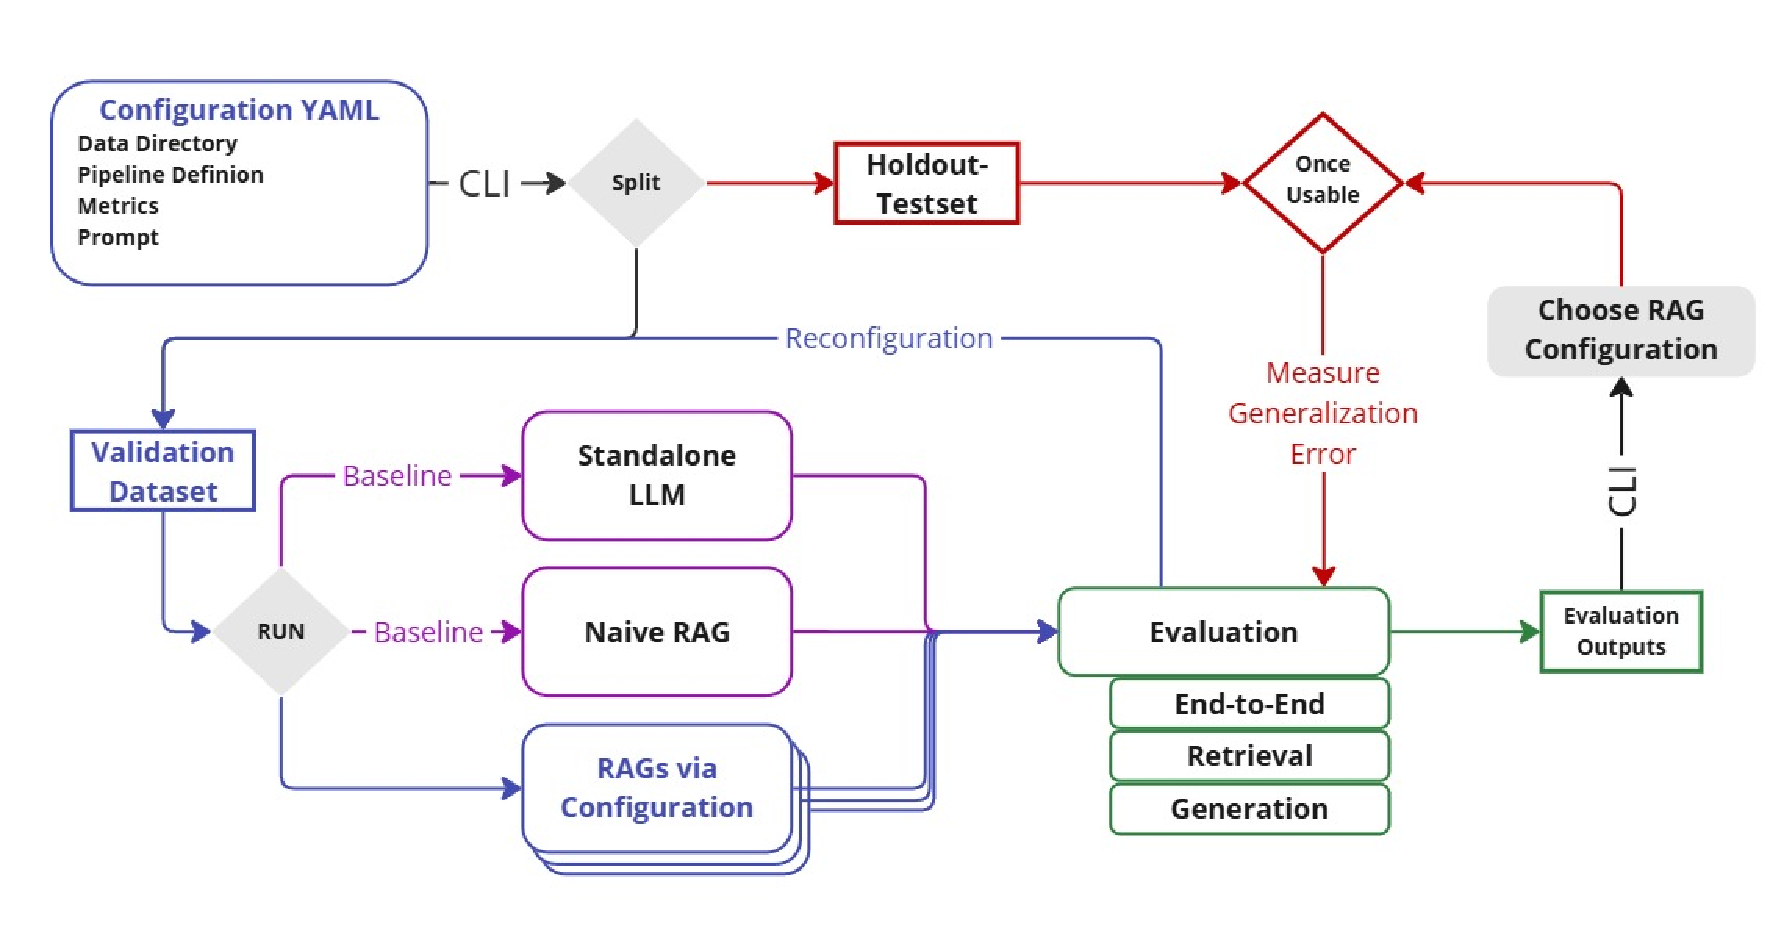
\includegraphics[width=\textwidth]{images/Sketch.pdf}
    \caption{...}
    \label{fig:EvaluationDesign}
\end{figure}


\section{Reproducibility of ML Experiments}
\begin{itemize}
    \item Seeding
    \item DVC 
    \item Logging all information
    \item Reporting
\end{itemize}

\section{Relevant Metrics for RAGs}
\begin{itemize}
    \item Task-specific vs Model-specific
    \item Performance vs System
    \item + Robust and Ethics
    \item Classification Metrics vs Generation Metrics
    \item RAGAS and Co. -> What do I need here?
\end{itemize}

\section{Coverage of Variety of RAG-Systems}

How I chose the right framework for it (Haystack vs Llama-Index vs Langchain)


